\documentclass[../main.tex]{subfiles}

\graphicspath{{\subfix{../figures}}}

\begin{document}

\section{Experiments}\label{sec:experiment}

This section presents a comprehensive experimental evaluation designed to validate the efficacy of our proposed cross-domain TNAS framework, \OUR{}.
We conduct a series of experiments across search spaces with different scales, providing in-depth analysis of the results.
Furthermore, to rigorously examine the individual components and design choices of our framework, we devise a set of studies for deeper analysis.
These studies serve to elucidate the contribution of each key element of our approach and to provide empirical support for our methodological decisions.

\subsection{Search Spaces and Datasets}

To assess the effectiveness of \OUR{}, a comprehensive set of experiments is designed, targeting three distinct NAS search spaces: NAS-Bench-201, NAS-Bench-101, and DARTS\@.
Each is selected to exemplify a different level of complexity and architectural constraints, providing a robust test bed for our methodologies.

\textbf{NAS-Bench-201 Space.}~\cite{DBLP:journals/pami/DongLMG22}\quad
This space employs a cell-based design where each architecture is depicted as a densely connected DAG\@.
It exclusively uses an OOE scheme, meaning that each edge in the DAG represents a specific operation
such as \texttt{NONE}, \texttt{SKIP-CONNECT}, \texttt{CONV-1X1}, \texttt{CONV-3X3},
or \texttt{AVG-POOL-3X3}, applied to the tensors flowing between nodes.
The NAS-Bench-201 contains a total of 15,625 unique architectures, each with 4 nodes, providing a compact yet comprehensive framework for initial testing of NAS algorithms.

\textbf{NAS-Bench-101 Space.}~\cite{DBLP:conf/icml/YingKCR0H19}\quad
Advancing in complexity, NAS-Bench-101 utilizes a cell-based architecture where each node in the DAG corresponds to an operation, conforming to an OON scheme.
Nodes represent different operations such as \texttt{CONV-3X3}, \texttt{CONV-1X1}, and \texttt{MAX-POOL-3X3}, with tensors as edges connecting these nodes.
This search space extends to architectures with at most 7 operators and no more than 9 connections, resulting in 423,624 unique configurations.
The increased expressiveness and complexity of the NAS-Bench 101 space challenge the adaptability and scalability of NAS solutions, making it serves as the complex domain.

\textbf{DARTS Space.}~\cite{DBLP:conf/iclr/LiuSY19}\quad
Representing much more complexity, DARTS features architectures as computational cells, each modeled as a DAG using an OOE scheme similar to NAS Bench-201 but with more advanced operational diversity.
Within each cell, the DAG consists of an ordered sequence of 7 nodes.
The first two nodes are designated as input tensors, while the last node serves as the output tensor.
The DARTS space includes sophisticated operations including \texttt{MAX-POOL-3X3}, \texttt{AVG-POOL-3X3}, \texttt{SKIP-CONNECT}, \texttt{SEP-CONV-3X3}, \texttt{SEP-CONV-5X5}, \texttt{DIL-CONV-3X3}, and \texttt{DIL-CONV-5X5}.
Two distinct cell types are employed: normal cells that preserve spatial resolution, and reduction cells that downsample the input feature maps.
DARTS space contains an expansive range of possibilities with over \num{e18} potential combinations of normal and reduction cells.
This space, serves as the challenging domain, tests the framework's capability to handle complex, large-scale environments and the effectiveness of solution transfers across highly varied architectural designs.

\begin{table}
  \centering
  \caption{Hyperparameter Configurations for Neural Architecture Representation Learning on Different Search Spaces}\label{tab:train-settings}
  \renewcommand*{\arraystretch}{1.3}
  \newcommand*{\sizefn}{\tabularnote{The number of samples used for training, represented in parentheses as their proportion to the entire search space. Same for other sizes.}}
  \newcommand*{\dartsfn}{\tabularnote{The DARTS search space encompasses a vast number of neural architectures, making it impractical to determine a specific proportion.}}
  \begin{NiceTabularX}{\linewidth}{@{}p{1.5cm}Xccc@{}}[notes,tabularnote={\textit{pt} = pre-training, \textit{ft} = fine-tuning, \textit{repr} = representation, \textit{ff} = feed-forward, \textit{enc-lyr} = encoder layer, \textit{dec-lyr} = decoder layer.}]
    \toprule
                                             &                             & \bfseries NB201 & \bfseries NB101 & \bfseries DARTS          \\
    \midrule\midrule
    \Block{4-1}{\bfseries Training Settings} & \textit{pt-size}\:\sizefn{} & 5,000~(0.5)     & 20,000~(0.5)    & 300,000~(--)\:\dartsfn{} \\
                                             & \textit{ft-size}            & 1,000~(0.1)     & 4,000~(0.01)    & 1,500~(--)               \\
    \cmidrule{2-5}
                                             & \textit{pt-epoch}           & 200             & 200             & 200                      \\
                                             & \textit{ft-epoch}           & 200             & 200             & 200                      \\
    \midrule\midrule
    \Block{6-1}{\bfseries Model Settings}    & \textit{repr-dim}           & 64              & 64              & 128                      \\
                                             & \textit{model-dim}          & 128             & 128             & 512                      \\
                                             & \textit{ff-dim}             & 256             & 256             & 2,048                    \\
    \cmidrule{2-5}
                                             & \textit{n-enc-lyr}          & 4               & 4               & 4                        \\
                                             & \textit{n-dec-lyr}          & 4               & 4               & 4                        \\
                                             & \textit{n-head}             & 4               & 4               & 4                        \\
    \bottomrule
  \end{NiceTabularX}
\end{table}

\subsection{Building Representations}

As discussed in Section~\ref{sec:method-build-repre}, representations for each search space are initially constructed.
Table~\ref{tab:train-settings} outlines the hyper-parameters employed for training the representation learners corresponding to each search space.
Training is conducted on a single NVIDIA RTX2080Ti.
We utilize the AdamW optimizer with a learning rate set to \num{2e-5} and a weight decay of \num{1e-6}.
Additionally, the scheduler used in~\cite{DBLP:conf/nips/VaswaniSPUJGKP17} is employed for adjusting the learning rate, with a warm-up period constituting 10\% of the total training steps.
The labels in the NAS-Bench-101 and NAS-Bench-201 spaces are derived from their respective benchmark datasets, whereas the DARTS space lacks a complete benchmark dataset. Therefore, we constructed the datasets for DARTS by training and collecting the necessary data.\footnote{This primarily includes the performance labels of neural architectures evaluated in our previous NAS processes, along with the training set from NAS-Bench-301.}

\begin{table}[t]
  \centering
  \caption{Comparative Performance Analysis of Neural Architecture Representation Learning Methods}\label{tab:repr-learn-metrics}
  \newcommand*{\trainfn}{\tabularnote{Distinct from other methodologies, our proposed approach maintains the flexibility of the encoder and decoder, enabling the integration of performance data into representation learning. This, however, results in a trade-off, with some reduction in reconstruction accuracy.}}
  \newcommand*{\dartsfn}{\tabularnote{The result is based on the labels we collected on the DARTS space.}}
  \begin{NiceTabularX}{\linewidth}{p{6em}lXcccc@{}}[notes]
    \toprule
                                                                   &                                               &                                                   & \bfseries NB201 & \bfseries NB101 & \bfseries DARTS  \\
    \midrule\midrule
    \Block{5-1}{\bfseries Reconstruction Accuray (\%)}             & \Block{5-1}{\bfseries\scriptsize\textuparrow} & \textit{arch2vec}~\cite{DBLP:conf/nips/YanZAZ020} & 99.99           & 98.84           & --               \\
                                                                   &                                               & SVGe~\cite{DBLP:conf/ijcnn/LukasikFZHK21}         & 99.99           & 99.57           & 99.63            \\
                                                                   &                                               & DGMG~\cite{DBLP:journals/corr/abs-1803-03324}     & 99.97           & 98.99           & 99.29            \\
    \cmidrule{3-6}
                                                                   &                                               & \OUR{} (Ptd.)                                     & 99.99           & 99.90           & 99.25            \\
                                                                   &                                               & \OUR{} (Ftd.)                                     & 99.06           & 99.99           & 99.12            \\
    \midrule\midrule
    \Block{4-1}{\bfseries Predicdtion Kendall's \( \bm{\tau} \)-b} & \Block{4-1}{\bfseries\scriptsize\textuparrow} & NAO~\cite{DBLP:conf/nips/LuoTQCL18}               & 0.526           & 0.775           & --               \\
                                                                   &                                               & TNASP~\cite{DBLP:conf/nips/LuLTYL21}              & 0.724           & 0.820           & --               \\
                                                                   &                                               & ReNAS-6~\cite{DBLP:conf/cvpr/Xu00TJX021}          & --              & 0.816           & --               \\
    \cmidrule{3-6}
                                                                   &                                               & \OUR{}                                            & \textbf{0.827}  & \textbf{0.848}  & 0.811~\dartsfn{} \\
    \bottomrule
  \end{NiceTabularX}
\end{table}

Table~\ref{tab:repr-learn-metrics} delineates the performance metrics of the proposed ternary representation learner. The initial section addresses the accuracy of reconstructing representations as inputs. High reconstruction accuracy signifies that the VAE effectively encapsulates the essential features of the input data. The findings demonstrate that the proposed method achieves reconstruction accuracies nearing 100\% across all three search spaces, indicating the construction of a sufficiently comprehensive representation of the neural architecture. It is noteworthy that the parameters of the VAE are not frozen, thereby allowing the performance information of the neural architecture to be integrated into the representation learning process. Consequently, there may have an unavoidable, yet acceptable, reduction in reconstruction accuracy.

The lower section of Table~\ref{tab:repr-learn-metrics} presents the results of fine-tuning with the ranker, concentrating on the rank correlation between the ranker's performance predictions and the ground truth labels.
The \textit{Kendall's \( \tau \)-b Correlation Coefficient}~(K-Tau) is employed to assess the ranker's capability to guide the transfer and search process.
The proposed predictor achieves coefficients of 0.809 in the NAS-Bench-101 space and 0.848 in the NAS-Bench-201 space, outperforming the methodologies introduced in NAO~\cite{DBLP:journals/corr/abs-1712-03351}, TNASP~\cite{E2EPPSun2023}, and ReNAS~\cite{DBLP:conf/cvpr/Xu00TJX021}.
Additionally, in the DARTS space, we achieve a sufficiently high K-Tau score as 0.811, supporting effective architecture transfer and search.
The results demonstrate that, with representation pre-training, our performance ranking predictor achieves superior accuracy and aligns more closely with the actual performance rankings.

It is crucial to highlight that the primary objective of this work is not to predict the performance of neural architectures. The aforementioned results demonstrate that the proposed method effectively extracts the intrinsic features of the neural architecture and is capable of making more accurate predictions of neural architecture performance. The representation learning underpin the fundamental theory of the proposed cross-domain transfer learning method for neural architectures.

\subsection{Transfer from Simple to Complex Domains}

\begin{figure}[t]
  \centering
  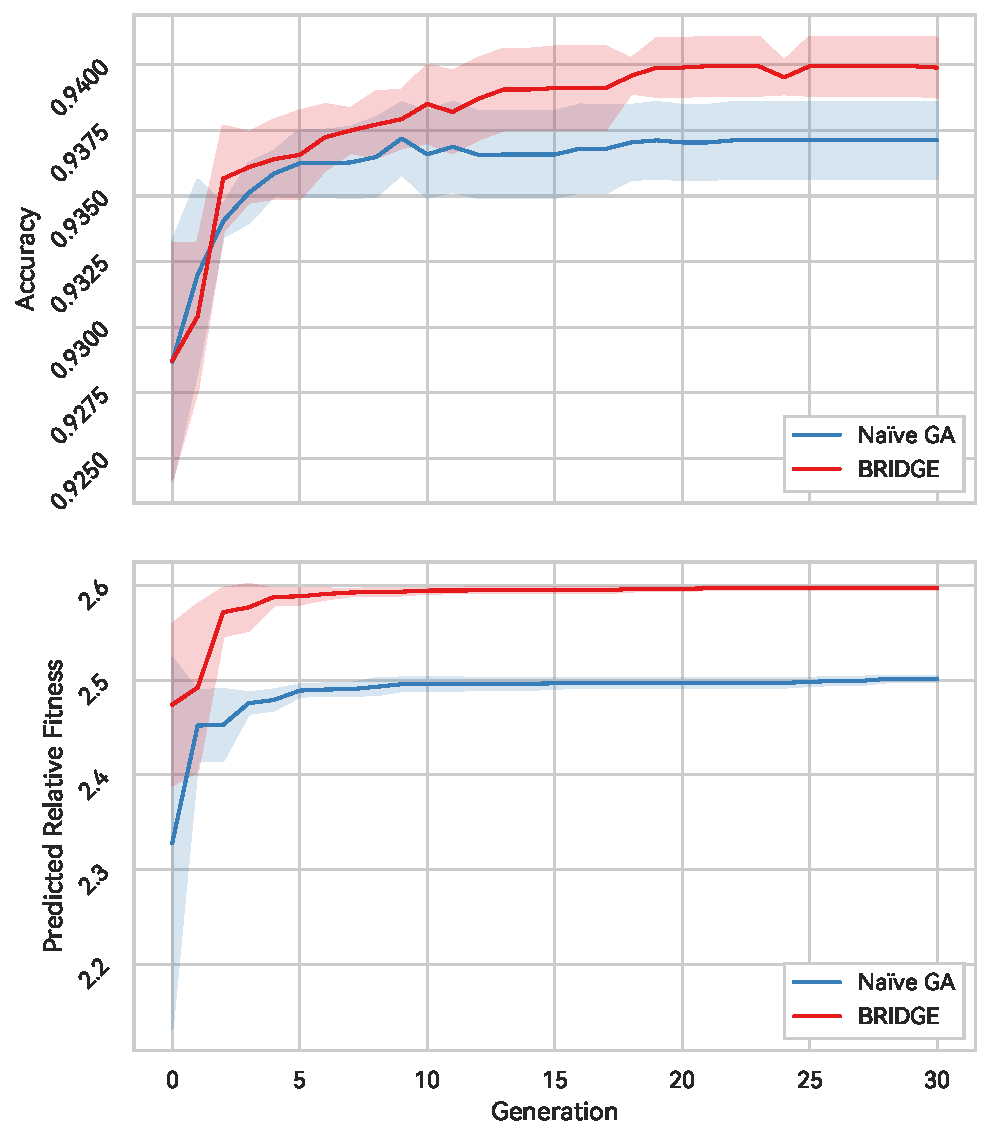
\includegraphics[width=\linewidth]{search-plot.pdf}
  \caption{
    Comparative analysis of evolutionary neural architecture search performance on NAS-Bench-101 with and without \OUR{}'s cross-domain ESTO mechanism.
    \ \textit{Top:} The ground truth accuracy of explored architectures over generations.
    \ \textit{Bottom:} Predicted relative fitness scores from the ranker module, which guides the NAS process as the evaluation strategy.
  }\label{fig:search-process-plot}
\end{figure}

\begin{table*}
  \centering
  \caption{Results of Neural Architecture Search on NAS-Bench-101 Space}\label{tab:transfer-result-101}
  \begin{NiceTabularX}{.8\linewidth}{X*{5}{c}}
    \toprule
    \bfseries Profile                         & \bfseries Optimal Acc. (\%) & \bfseries Average Acc. (\%) & \bfseries \#Evaluation & \bfseries Method Type   \\
    \midrule\midrule
    ENAS~\cite{pham_efficient_2018}           & 92.54                       & 91.83\( \pm \)0.61          & --                  & weight sharing          \\
    FBNet~\cite{DBLP:conf/cvpr/WuDZWSWTVJK19} & 93.98                       & 92.29\( \pm \)1.84          & --                  & gradient-based          \\
    CTNAS~\cite{DBLP:conf/cvpr/ChenGCLZWT21}  & 94.14                       & 93.93\( \pm \)0.42          & --                  & predictor               \\
    ReNAS~\cite{DBLP:conf/cvpr/Xu00TJX021}    & 94.07                       & 93.95\( \pm \)1.25          & 423                 & predictor               \\
    SVGe~\cite{DBLP:conf/ijcnn/LukasikFZHK21} & 93.88                       & --                          & --                  & representation learning \\
    \midrule
    \RowStyle[nb-rows=4,color=BrickRed]{}
    PSO                                       & 93.77                       & 93.71\( \pm \)0.04          
    & --                  & \\ 
    PSO+\OUR{}                                & 93.96                       & 93.92\(  \pm\)0.04          & --                  & \\
    MA & 94.07 & 93.93\( \pm \)0.36 & -- & \\
    MA+\OUR{} & 94.32 & 94.02\( \pm \)0.12 & -- & \\
    \midrule
    Na{\"\i}ve GA (baseline)                  & 93.96                       & 93.71\( \pm \)1.74          & 500                 & representation learning \\
    \OUR{} (ours)                             & \textbf{94.17}              & \textbf{93.99}\( \pm \)1.56 & 400                 & representation learning \\
    \bottomrule
  \end{NiceTabularX}
\end{table*}

We conducted preliminary validation of the proposed method through experiments involving transfer learning from simple to complex domains, specifically using solutions from the NAS-Bench-201 space to enhance the search in the NAS-Bench-101 space.
The mapping matrix \( \mathcal{M} \) is constructed by sampling 1,000 solutions from the training sets of both sides separately.
We selected Genetic Algorithm~(GA)~\cite{HollandGA1992}, a widely used method in NAS, as the evolutionary search solver.
Following the settings in~\cite{DBLP:conf/iconip/HouDFQ21}, the GA solver used a population size of 20, with \textit{Single Point Crossover} and \textit{Polynomial Mutation}, both set at a probability of 0.5, and \textit{Binary Tournament Selection}.

The results, presented in Table~\ref{tab:transfer-result-101}, compare our method against a baseline established by the same GA solver but excluding the proposed cross-domain transfer method (Na{\"i}ve GA).
Our findings significantly outperform the baseline, showing notable improvements in both optimal and average accuracy metrics, with values of 94.17\% and 93.99\%, respectively. This demonstrates the effectiveness of our transfer learning approach.
Furthermore, our method outperforms the majority of existing predictor-based NAS methods and can be integrated with these approaches to achieve even more robust outcomes.

To further illustrate the impact of transfer learning on the search process, Fig.~\ref{fig:search-process-plot} shows the generation-by-generation trend of the population's optimal solution. In the early stages, the transferred solutions create a high-quality and diverse initial population, thus enabling the exploration of more optimal solution regions from the onset. In summary, our proposed transfer learning method effectively accelerates the process of neural architecture search, allowing it to converge earlier to a better result region.


\subsection{Transfer to More Challenging Domains}

To further assess the robustness of our transfer learning framework, we extended our evaluation to more challenging domains, specifically focusing on the DARTS space.
This space represents a highly complex search environment, as previously discussed.
The DARTS space presents significant challenges compared to NAS-Bench-101 and NAS-Bench-201, encompassing a broader range of optional operations, a greater number of operations per cell, and notably, a combination of two distinct cell types.
These substantial differences between domains pose considerable challenges for transfer learning, making this evaluation particularly rigorous.

Our experimental setup involves transferring knowledge from the NAS-Bench-101 space to inform and enhance the search within the DARTS space.
Table~\ref{tab:transfer-result-301} summarizes the performance of our approach in comparison to baseline methods.
Notably, our proposed \OUR{} achieved an accuracy of 97.33\%, significantly outperforming the baseline approaches.
This result demonstrates our method's capacity to effectively transfer and adapt knowledge to complex domains.
To provide an additional performance metric, we utilize the performance predictor from NAS-Bench-301 to evaluate our discovered architecture.
This auxiliary measure offers further validation of our approach's efficacy within the DARTS space.

These results underscore the adaptability of our method to varied and complex architectural designs.
This adaptability is crucial for addressing the challenges posed by large-scale search spaces, thus validating the practical applicability of our framework in real-world scenarios.
Moreover, the successful transfer across domains with high dissimilarity suggests that our representation learning approach effectively extracts the underlying semantic information of neural architectures.
This capability to bridge disparate domains could significantly advance the field of automated machine learning, enabling more efficient and effective architecture discovery across a wide range of tasks and domains.

\begin{table}
  \centering
  \caption{Results of Neural Architecture Search on DARTS Space}\label{tab:transfer-result-301}
  \begin{NiceTabularX}{.95\linewidth}{X*{3}{>{\centering\arraybackslash}p{5em}}}
    \toprule
    \bfseries Profile        & \Block{1-1}{\bfseries Optimal Acc. (\%)} & \Block{1-1}{\bfseries NB301 Prediction} & \bfseries \#Queries \\
    \midrule\midrule
    Na{\"\i}ve GA (baseline) & 96.62                                    & 94.85                                   & 600                 \\
    \OUR{} (ours)            & \bfseries 97.33                          & \bfseries 94.93                         & 600                 \\
    \bottomrule
  \end{NiceTabularX}
\end{table}

\subsection{Deeper Analysis}

\subsubsection{Hyperparameter Sensitivity Analysis}\label{sec:hyperparam-analysis}

\begin{figure}
  \centering
  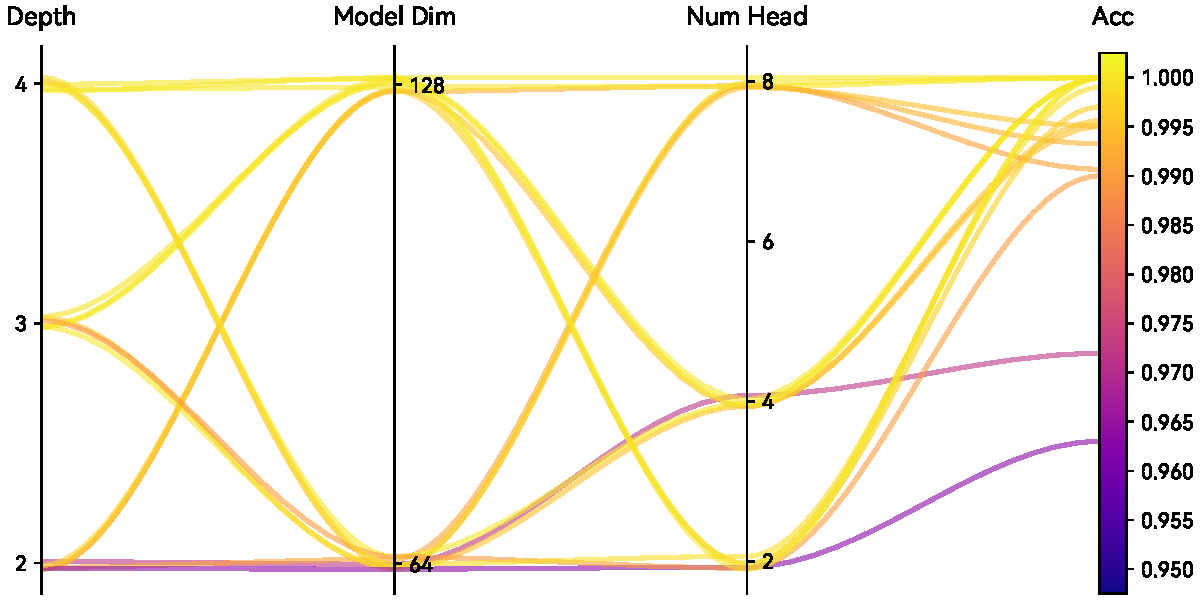
\includegraphics[width=.95\linewidth]{hpsa.pdf}
  \DiffBegin
  \caption{
    Parallel coordinates plot showing the accuracy of the proposed representation learner on NAS-Bench-101 under different hyperparameter settings.
    Each line corresponds to a unique combination of network depth, model dimension, and number of attention heads, while the color scale indicates the resulting accuracy (darker lines indicate lower accuracy and brighter lines indicate higher accuracy).
  }\label{fig:hyperparam-sensitivity}
  \DiffEnd
\end{figure}

\subsubsection{Latent Representation Space Observation}\label{sec:repre-space-analysis}

To provide a more intuitive representation of the evolving distribution within the latent representation space throughout the training process, we employ \textit{Multi-Dimensional Scaling} (MDS)~\cite{DOUGLASCARROLL1998179} for visualization.
Additionally, we color-code the sampled points according to their ground-truth labels to facilitate interpretation.
As illustrated in Fig.~\ref{fig:nb101-mds}, neural architectures with similar performance metrics exhibit spatial proximity within the latent representation space across various stages of the representation learning process.
This aggregation demonstrates a gradual, stepwise increase in coherence over training process.

The observed clustering behavior aligns with the inherent properties of VAEs. During the pre-training phase, the VAE naturally tends to position similar neural architectures in close proximity within the latent space. Moreover, architectures with structural similarities have a higher probability of exhibiting comparable performance characteristics. This intrinsic organization provides a robust foundation for the subsequent training of the performance ranker.
In the fine-tuning phase, the introduction of supervisory signals derived from ground-truth labels further enhances the model's capacity to capture features that contribute to performance differentials. This refinement is reflected in the latent space distribution, where representations of neural architectures with similar performance metrics display remarkable aggregation.

\begin{figure}
  \centering
  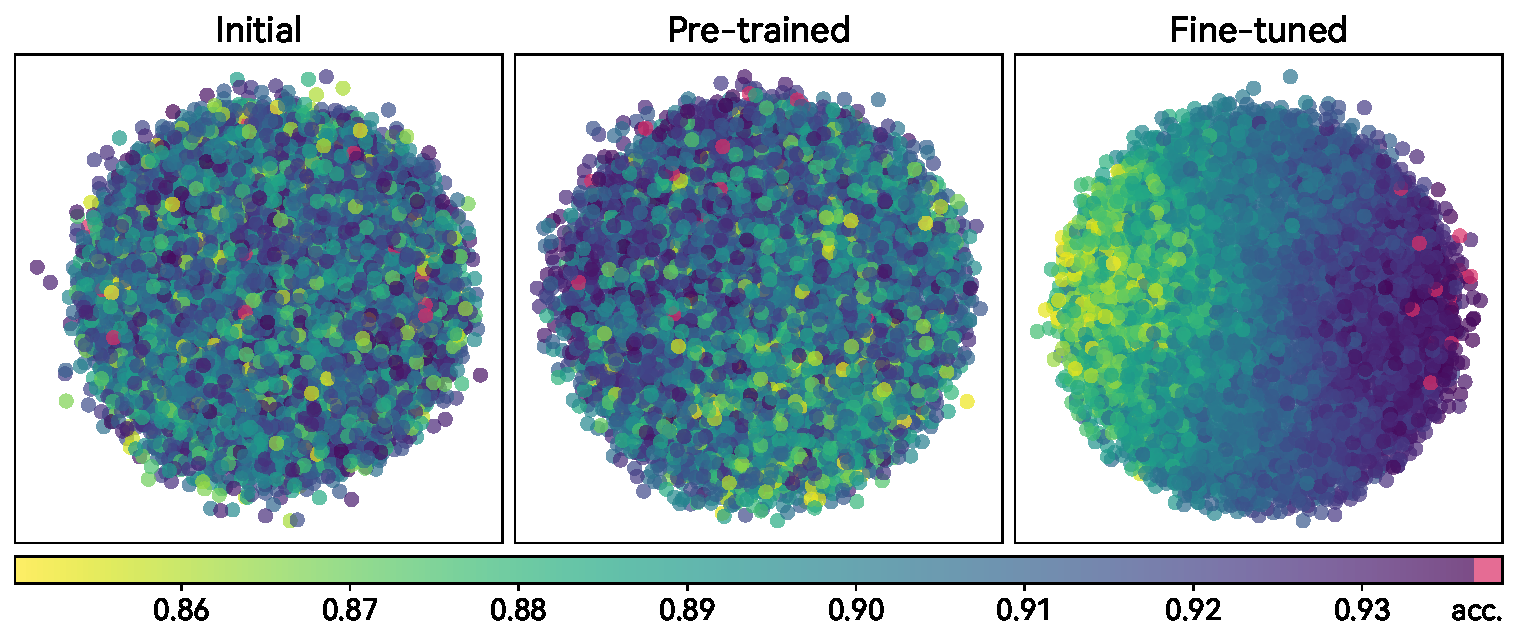
\includegraphics[width=.95\linewidth]{nb101-mds.pdf}
  \caption{
    Visualization of the learned representation space for NAS-Bench-101 architectures across different training stages: initial (left), after pre-training (middle), and after fine-tuning (right).
    Colors indicate architecture performance (accuracy), with warmer colors representing higher accuracy.
  }\label{fig:nb101-mds}
\end{figure}

\subsubsection{The Impact of The Amount of Training Data Used}

\begin{table}
  \centering
  \caption{Neural Architecture Representation Learning Performance During the Pretrain Stage on NAS-Bench-101, Evaluated Across Different Dataset Sizes}\label{tab:ablation-pretrin-data-size}
  \newcommand*{\ablationfn}{\tabularnote{In order to eliminate the interference of predictor in the experiment, we use a unified performance predictor among dataset sizes.}}
  \begin{NiceTabularX}{\linewidth}{p{12em}*{5}{>{\centering\arraybackslash}X}}
    \toprule
    \bfseries Unlabeled Data & \bfseries 1\% & \bfseries 5\% & \bfseries 10\% & \bfseries 30\% & \bfseries 50\% \\
    \midrule\midrule
    \textbf{VAE Acc.} (\%)   & 78.82         & 89.46         & 99.91          & 99.56          & 99.97          \\
    \textbf{Cost} (GPU Days) & 0.08          & 0.08          & 0.08           & 0.11           & 0.15           \\
    \bottomrule
  \end{NiceTabularX}
\end{table}

\begin{table}
  \centering
  \caption{Neural Architecture Representation Learning Performance During the Finetuning Stage on NAS-Bench-101, Evaluated Across Different Dataset Sizes}\label{tab:ablation-finetune-data-size}
  \newcommand*{\ablationfn}{\tabularnote{In order to eliminate the interference of predictor in the experiment, we use a unified performance predictor among dataset sizes.}}
  \begin{NiceTabularX}{\linewidth}{p{12em}*{3}{>{\centering\arraybackslash}X}}
    \toprule
    \bfseries Labeled Data              & \bfseries 0.1\% & \bfseries 1\% & \bfseries 5\% \\
    \midrule\midrule
    \bfseries Kendall's \(\bm{\tau}\)-b & 0.738           & 0.848         & 0.865         \\
    \bfseries Cost (GPU Days)           & 0.01            & 0.02          & 0.02          \\
    \textbf{Optimal Result}             &                 &               &               \\
    \quad --- As Source (\%)            & 96.56           & 97.33         & 97.36         \\
    \quad --- As Target (\%)            & 93.68           & 94.17         & 94.24         \\
    \bottomrule
  \end{NiceTabularX}
\end{table}
The representation learning model constitutes a fundamental component of our proposed transfer framework, playing a significant role in the effectiveness of knowledge transfer and, consequently, in determining the performance outcomes.
.Our training methodology for the representation learning model comprises two phases: unsupervised pre-training followed by supervised fine-tuning.
As discussed in Section~\ref{sec:repre-space-analysis}, the fine-tuning phase is particularly important for aligning cross-domain representation spaces. Given the critical influence of labeled data on model fine-tuning, we conducted an investigation into the effects of varying data ratios on neural architecture representation learning on NAS-Bench-101.

Table~\ref{tab:ablation-pretrin-data-size} presents key performance indicators of neural architecture representation learning across a range of dataset sizes.
During fine-tuning, the VAE shows robust performance across different dataset sizes, achieving accuracies of at least 99.90\%, indicating that it can consistently capture the underlying structure of neural architectures even with limited data.
This suggests that unsupervised learning effectively models architectural features despite variations in data volume.
However, the performance of the predictor component demonstrates greater sensitivity to the amount of training data.
As dataset size increases, K-Tau improves, reaching a maximum value of 0.862 at 5\% of the dataset, reflecting stronger predictive performance with larger datasets.

This sensitivity manifests not only in prediction accuracy but also influences the distribution characteristics of the learned representation space.
Our findings indicate that larger labeled datasets contribute to a more structured and well-organized representation space, facilitating the learning of more precise mapping functions between domains. This improved structure and increased accuracy in inter-domain mapping directly enhance search performance on target tasks.
For example, with 5\% of the total dataset, we achieve accuracies of 97.36\% as the source domain and 94.24\% as the target domain, illustrating the benefits of larger datasets for cross-domain transferability.

In summary, while the VAE demonstrates resilience to limited data, the performance predictor and transfer learning stages benefit significantly from larger datasets. This highlights the importance of data acquisition and curation in transfer learning scenarios, particularly when aiming to optimize performance in target domains with limited labeled data.

\end{document}